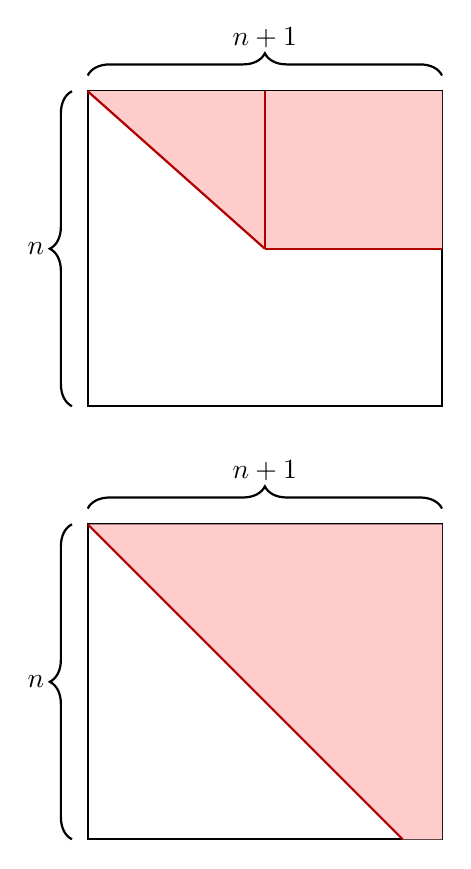
\begin{tikzpicture}[
    every node/.style={inner sep=0pt, outer sep=0pt},
    % Stile per le graffe
    curlybrace/.style={
        thick,
        decoration={brace, amplitude=8pt},
        decorate
    },
    % Stile per i bordi delle matrici
    matrixbox/.style={
        draw=black,
        thick,
        fill=white
    }
]

% Dimensioni generali (puoi scalarle modificando questi valori)
\def\matH{4}   % Altezza (n)
\def\matW{4.5} % Larghezza (n+1)

% ================================
% MATRICE SUPERIORE (FASE INTERMEDIA)
% ================================
\begin{scope}
    % Bordo esterno
    \draw[matrixbox] (0,0) rectangle (\matW,\matH);
    
    % Area ombreggiata (triangolo + rettangolo)
    \fill[fill=red!20] (0,\matH) -- (\matW/2,\matH/2) -- (\matW,\matH/2) -- (\matW,\matH) -- cycle;
    
    % Linee rosse interne
    \draw[draw=red!70!black, thick] (0,\matH) -- (\matW/2,\matH/2); % Diagonale
    \draw[draw=red!70!black, thick] (\matW/2,\matH/2) -- (\matW,\matH/2); % Orizzontale
    \draw[draw=red!70!black, thick] (\matW/2,\matH/2) -- (\matW/2,\matH); % Verticale
    
    % Graffe e label
    \draw[curlybrace] (-0.2,0) -- (-0.2,\matH) node[midway, left=10pt] {$n$};
    \draw[curlybrace] (0,\matH+0.2) -- (\matW,\matH+0.2) node[midway, above=10pt] {$n+1$};
\end{scope}

% ================================
% MATRICE INFERIORE (REF COMPLETATA)
% ================================
\begin{scope}[yshift=-5.5cm] % Sposta la seconda matrice verso il basso
    % Bordo esterno
    \draw[matrixbox] (0,0) rectangle (\matW,\matH);
    
    % Area ombreggiata (tutta la parte superiore + colonna extra)
    % La diagonale scende da (0,H) fino alla base (H,0) assumendo un blocco quadrato n x n
    \fill[fill=red!20] (0,\matH) -- (\matH,0) -- (\matW,0) -- (\matW,\matH) -- cycle;
    
    % Linea rossa della diagonale principale
    \draw[draw=red!70!black, thick] (0,\matH) -- (\matH,0);
    
    % Graffe e label
    \draw[curlybrace] (-0.2,0) -- (-0.2,\matH) node[midway, left=10pt] {$n$};
    \draw[curlybrace] (0,\matH+0.2) -- (\matW,\matH+0.2) node[midway, above=10pt] {$n+1$};
\end{scope}

\end{tikzpicture}